


\begin{frame}{Энкодер-агностичные модели: перенос знаний между языками}
%\resizebox{\textwidth}{!}
\scalebox{0.48}{
\begin{tabular}{|c|c|c||c|c|c|c|c|c|} \hline
Модель & \begin{tabular}[c]{@{}l@{}}Тренировочные\\данные\end{tabular} & Режим & Среднее & \begin{tabular}[c]{@{}l@{}}Эмоции\end{tabular} & \begin{tabular}[c]{@{}l@{}}Тональность\end{tabular} & \begin{tabular}[c]{@{}l@{}}Токсичность\end{tabular} & \begin{tabular}[c]{@{}l@{}}Интенты\end{tabular} & \begin{tabular}[c]{@{}l@{}}Темы\end{tabular} \\
\hline \hline
\textit{distilbert-mult} & RU & S & 84.7 & 77.4 & 77.7 & 96.7 & 83.5 & 88.1 \\ %\hline
\textit{distilbert-mult} & RU & M & 84.3 & 78.1 & 76.8 & 96.5 & 81.9 & 88.2  \\ \hline
\textit{distilbert-mult} & \begin{tabular}[c]{@{}l@{}}RU+EN,\\объединенные\end{tabular} & S & 85.2 & 78.9 & 77.4 & 96.8 & 84.7 & 88.4 \\ %\hline
\textit{distilbert-mult} & \begin{tabular}[c]{@{}l@{}}RU+EN,\\объединенные\end{tabular} & M & 84.5 & 77.9 & 76.6 & 96.5 & 82.9 & 88.4 \\ \hline
\textit{distilbert-mult} & \begin{tabular}[c]{@{}l@{}}RU+EN,\\отдельные\end{tabular} & M & 84.4 & 77.6 & 76.8 & 96.5 & 82.4 & 88.3 \\ \hline
\textit{bert-mult} & RU & S & 84.7 & 76.6 & 77.8 & 96.9 & 83.9 & 88.4 \\ %\hline
\textit{bert-mult} & RU & M & 84.8 & 78.4 & 76.3 & 96.8 & 83.7 & 89.0 \\ \hline
\textit{bert-mult} & \begin{tabular}[c]{@{}l@{}}RU+EN,\\объединенные\end{tabular} & S & 85.6 & 78.9 & 77.6 & 96.9 & 85.0 & 89.4 \\ %\hline
\textit{bert-mult} & \begin{tabular}[c]{@{}l@{}}RU+EN,\\объединенные\end{tabular} & M & 85.2 & 79.2 & 76.4 & 96.7 & 84.3 & 89.4 \\ \hline
\textit{bert-mult} & \begin{tabular}[c]{@{}l@{}}RU+EN,\\отдельные\end{tabular} & M & 85.0 & 78.3 & 77.1 & 96.7 & 84.0 & 89.1 \\ \hline
\end{tabular}}

\end{frame}

\begin{frame}{Точность при кросс-валидации}
\scalebox{0.5}{
\label{tab:crossvalidation}
\begin{tabular}{|c||c|c|c|c|c|c|c|c|c|c|c|c|}
\hline
\multirow{2}{*}{\textbf{Модель}} & \multicolumn{2}{c|}{\textbf{Среднее}} & \multicolumn{2}{c|}{\textbf{Разб. 1}} & \multicolumn{2}{c|}{\textbf{Разб. 2}} &\multicolumn{2}{c|}{\textbf{Разб. 3}} & \multicolumn{2}{c|}{\textbf{Разб. 4}} & \multicolumn{2}{c|}{\textbf{Разб. 5}} \\ 
\cline{2-13}
& Точность & Макро-F1 & Точность & Макро-F1 & Точность & Макро-F1 & Точность & Макро-F1   & Точность & Макро-F1 & Точность & Макро-F1 \\ \hline
%\textit{rusber} & 74.0 & 53.4 \\ \hline
%\textit{ru} & 73.7 & 52.5 \\ \hline
%\textit{rutiny} & 72.2 & 50.9 \\ \hline
%\textit{mult} & 71.4 & 51.9 \\ \hline
\textit{rusber} & 74.0 & 53.4 & 73.7 & 54.3 & 73.8 & 52.8 & 73.9 & 53.0 & 74.1 & 54.2 & 74.2 & 52.9\\
\textit{ru} & 73.7 & 52.5 & 73.5 & 52.9 & 73.7 & 51.9 & 73.6 & 52.3 & 73.9 & 53.1 & 73.9 & 52.3\\
\textit{rutiny} & 72.2 & 50.9 & 72.0 & 49.7 & 72.2 & 50.9 & 72.0 & 51.4 & 72.4 & 51.1 & 72.3 & 51.6\\
\textit{mult} & 71.4 & 51.9 & 71.2 & 52.4 & 71.5 & 51.9 & 71.5 & 51.4 & 71.2 & 51.6 & 71.7 & 52.1\\ \hline
\end{tabular}
}
\end{frame}


\begin{frame}{4. Многоязычный перенос знаний: между всеми языками из MASSIVE - выводы}
%TODO p-value p-значение
Корреляция Спирмена точности для каждого языка с приближенным размером обучающей выборки равняется 0.773 (p-значение 5.02e-10). При этом корреляция точности с генеалогической дистанцией до русского равна -0.323 (p-значение 0.022). 
\newline 
\newline Если принять в расчёт при подсчете этой корреляции приближенный размер обучающей выборки как третью переменную, то частичная корреляция точности с генеалогической дистанцией до русского языка становится равной -0.151 с пи-значением 0.3, что не является статистически значимым.

\end{frame}



\begin{frame}{Энкодер-агностичные модели - эффект уменьшения размера выборки по задачам}

\begin{figure}[!ht]
\begin{subfigure}{0.3\textwidth}
\begin{tikzpicture}[scale=1]
\begin{axis}[xlabel = Число тренировочных примеров,
ylabel = Точность,
title=Средняя точность,
legend pos= south east,
width=\textwidth,
% width=10cm,
% height=10cm,
% xmin=2,
% xmax=100,
xtick={0,1,2,3,4,5,6,7},
xticklabels={6k,10k,21k,31k,41k,51k,103k,205k},
ymin=50,ymax=90,
legend cell align={left},
legend style={nodes={scale=0.5, transform shape}}
]
\addplot[color=orange,dotted, mark=*] coordinates {
(0, 57.02)
(1, 58.379999999999995)
(2, 75.66666666666667)
(3, 77.7)
(4, 78.36666666666667)
(5, 79.53333333333333)
(6, 82.5)
(7, 84.39999999999999)
};
\addlegendentry{Однозадачная точность (RU)}
\addplot[color=red,solid,mark=*] coordinates {
(0, 65.88)
(1, 70.3)
(2, 75.23333333333333)
(3, 77.23333333333333)
(4, 79.0)
(5, 79.60000000000001)
(6, 82.3)
(7, 84.33333333333333)};
\addlegendentry{Многозадачная точность (RU)}
\end{axis}
\end{tikzpicture}
\end{subfigure}
\begin{subfigure}{0.3\textwidth}
\begin{tikzpicture}[scale=1]
\begin{axis}[xlabel = Число обучающих примеров,
ylabel = Точность,
title=Классификация эмоций,
legend pos= south east,
width=\textwidth,
% width=10cm,
% height=10cm,
% xmin=2,
% xmax=100,
xtick={0,1,2,3,4,5,6,7},
xticklabels={196, 327, 655, 983, 1311, 1639, 3278, 6557},
ymin=45,ymax=80,
legend cell align={left},
legend style={nodes={scale=0.5, transform shape}}
]
\addplot[color=orange,dotted, mark=*] coordinates {
(0, 49.14)
(1, 48.260000000000005)
(2, 64.5)
(3, 66.10000000000001)
(4, 64.26666666666667)
(5, 66.96666666666665)
(6, 73.96666666666667)
(7, 76.46666666666667)
};
\addlegendentry{Однозадачная точность (RU)}
\addplot[color=red,solid,mark=*] coordinates {
(0, 62.61999999999999)
(1, 64.82000000000001)
(2, 68.73333333333333)
(3, 70.73333333333333)
(4, 71.36666666666667)
(5, 72.3)
(6, 75.0)
(7, 78.13333333333334)};
\addlegendentry{Многозадачная точность (RU)}
\end{axis}%
\end{tikzpicture}
\end{subfigure}

\medskip

\begin{subfigure}{0.3\textwidth}
\begin{tikzpicture}[scale=1]
\begin{axis}[xlabel = Число обучающих примеров,
ylabel = Точность,
title=Классификация тональности,
legend pos= south east,
width=\textwidth,
% width=10cm,
% height=10cm,
% xmin=2,
% xmax=100,
xtick={0,1,2,3,4,5,6,7},
xticklabels={2k, 4k, 8k, 12k, 17k, 21k, 41k, 83k},
ymin=65,ymax=80,
legend cell align={left},
legend style={nodes={scale=0.5, transform shape}}
]
\addplot[color=orange,dotted, mark=*] coordinates {
(0, 69.46000000000001)
(1, 71.02000000000001)
(2, 73.3)
(3, 73.96666666666665)
(4, 74.36666666666666)
(5, 75.13333333333334)
(6, 76.36666666666667)
(7, 77.16666666666667)
};
\addlegendentry{Однозадачная точность (RU)}
\addplot[color=red,solid,mark=*] coordinates {
(0, 68.99999999999999)
(1, 70.14)
(2, 71.46666666666665)
(3, 71.7)
(4, 72.96666666666667)
(5, 72.66666666666667)
(6, 74.56666666666666)
(7, 76.23333333333333)};
\addlegendentry{Многозадачная точность (RU)}
\end{axis}%
\end{tikzpicture}
\end{subfigure}
\begin{subfigure}{0.3\textwidth}
\begin{tikzpicture}[scale=1]
\begin{axis}[xlabel = Число обучающих примеров,
ylabel = Точность,
title=Классификация токсичности,
legend pos= south east,
width=\textwidth,
% width=10cm,
% height=10cm,
% xmin=2,
% xmax=100,
xtick={0,1,2,3,4,5,6,7},
xticklabels={3k, 5k, 9k, 14k, 19k, 23k, 47k, 93k},
ymin=90,ymax=100,
legend cell align={left},
legend style={nodes={scale=0.5, transform shape}}
]
\addplot[color=orange,dotted, mark=*] coordinates {
(0, 91.50000000000001)
(1, 92.70000000000002)
(2, 93.93333333333334)
(3, 94.80000000000001)
(4, 95.06666666666666)
(5, 95.36666666666667)
(6, 96.13333333333333)
(7, 96.7)
};
\addlegendentry{Однозадачная точность (RU)}
\addplot[color=red,solid,mark=*] coordinates {
(0, 91.24000000000001)
(1, 92.6)
(2, 93.96666666666665)
(3, 94.60000000000001)
(4, 95.0)
(5, 95.33333333333333)
(6, 96.0)
(7, 96.5)};
\addlegendentry{Многозадачная точность (RU)}
\end{axis}%
\end{tikzpicture}
\end{subfigure}

\medskip

\begin{subfigure}{0.3\textwidth}
\begin{tikzpicture}
\begin{axis}[xlabel = Число обучающих примеров,
ylabel = Точность,
title=Классификация интентов,
legend pos= south east,
width=\textwidth,
% width=10cm,
% height=10cm,
% xmin=2,
% xmax=100,
xtick={0,1,2,3,4,5,6,7},
xticklabels={0.3k, 0.6k, 1.2k, 1.7k, 2.3k, 2.9k, 5.8k, 11.5k},
ymin=25,ymax=85,
legend cell align={left},
legend style={nodes={scale=0.5, transform shape}}
]
\addplot[color=orange,dotted, mark=*] coordinates {
(0, 38.9)
(1, 29.920000000000005)
(2, 67.7)
(3, 72.16666666666667)
(4, 75.33333333333333)
(5, 76.60000000000001)
(6, 79.96666666666668)
(7, 83.46666666666665)
};
\addlegendentry{Однозадачная точность (RU)}
\addplot[color=red,solid,mark=*] coordinates {
(0, 42.64)
(1, 52.98)
(2, 64.03333333333335)
(3, 68.6)
(4, 73.5)
(5, 73.83333333333333)
(6, 79.5)
(7, 82.36666666666667)};
\addlegendentry{Многозадачная точность (RU)}
\end{axis}
\end{tikzpicture}
\end{subfigure}
\begin{subfigure}{0.3\textwidth}
\begin{tikzpicture}
\begin{axis}[xlabel = Число обучающих примеров,
ylabel = Точность,
title=Тематическая классификация,
legend pos= south east,
width=\textwidth,
% width=10cm,
% height=10cm,
% xmin=2,
% xmax=100,
xtick={0,1,2,3,4,5,6,7},
xticklabels={0.3k, 0.6k, 1.2k, 1.7k, 2.3k, 2.9k, 5.8k, 11.5k},
ymin=35,ymax=90,
legend cell align={left},
legend style={nodes={scale=0.5, transform shape}}
]
\addplot[color=orange,dotted, mark=*] coordinates {
(0, 36.16)
(1, 50.06)
(2, 78.80000000000001)
(3, 81.56666666666666)
(4, 82.86666666666666)
(5, 83.60000000000001)
(6, 86.13333333333334)
(7, 88.2)
};
\addlegendentry{Однозадачная точность (RU)}
\addplot[color=red,solid,mark=*] coordinates {
(0, 42.64)
(1, 52.98)
(2, 64.03333333333335)
(3, 68.6)
(4, 73.5)
(5, 73.83333333333333)
(6, 79.5)
(7, 82.36666666666667)};
\addlegendentry{Многозадачная точность (RU)}
\end{axis}%
\end{tikzpicture}
\end{subfigure}


\caption{Однозадачная и многозадачная точность для каждой задачи. Русский язык.}
\label{fig:tr-ag:ru_dialog_part_n_samples}
\end{figure}
\end{frame}


\begin{frame}{4. Многоязычный перенос знаний: главные выводы из тестирования данных}
\begin{enumerate}
\item Модели, учившиеся только на ответах, показывают лучшие результаты, чем учившиеся только на вопросах, а учившиеся только на ответах. Это верно для всех рассмотренных базовых моделях, что доказывает: вопросы -- самый информативный элемент набора данных {RuQTopics}. 

\item Конкатенация вопросов к ответам не дает стойкого улучшения по сравнению с использованием только лишь вопросов. 

\item В общем и целом, все русскоязычные модели показывают похожие результаты, а многоязычная модель ожидаемо показывает результаты хуже, чем любая из русскоязычных. 

\item Все эти выводы также справедливы для экспериментов, в которых использовались все данные из части 1 набора данных {RuQTopics}, принадлежащие вышеупомянутым шести классам.
\end{enumerate}
\end{frame}


\begin{frame}{5. Диалоговая платформа Dream: архитектура в конкурсе «Alexa Prize Challenge 3»}
    \centering
    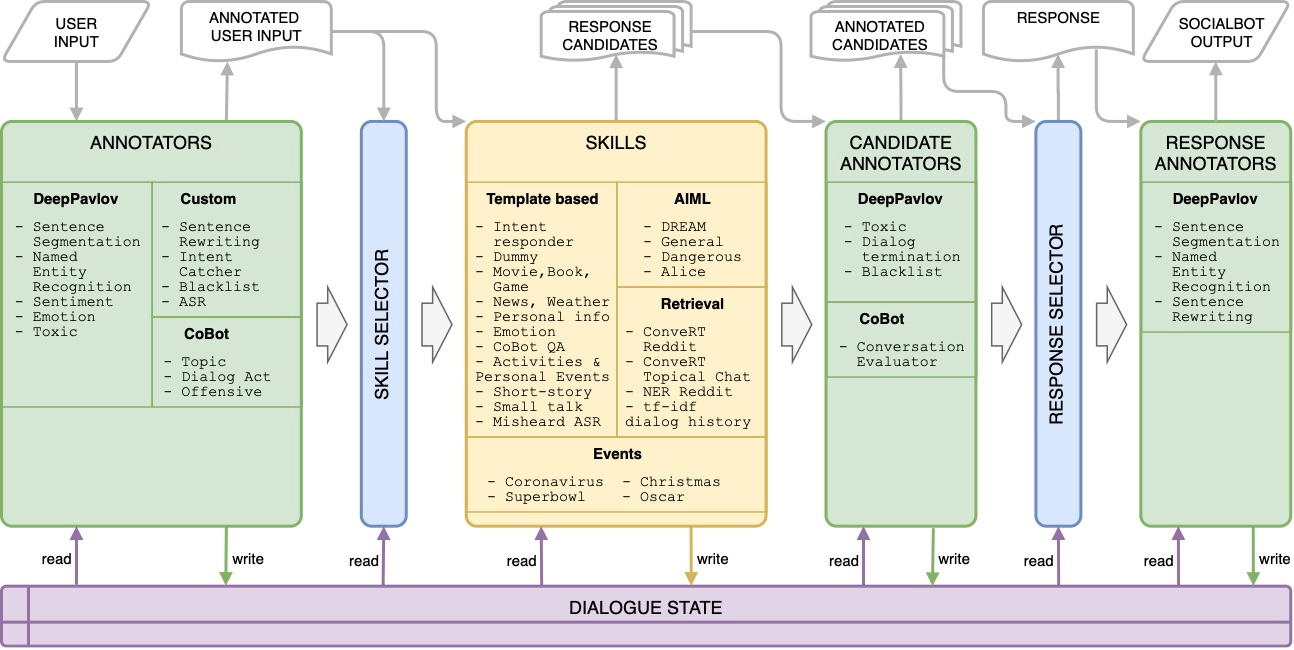
\includegraphics[width=1\linewidth]{images/Alexa1_.png} 
\end{frame}
